\subsection{相交线、对顶角}\label{subsec:czjh1-2-1}

交叉的道路、管道(图 \ref{fig:czjh1-2-1}) 等都给我们以相交直线的形象。

\begin{figure}[htbp]
    \centering
    \begin{minipage}[b]{7cm}
        \centering
        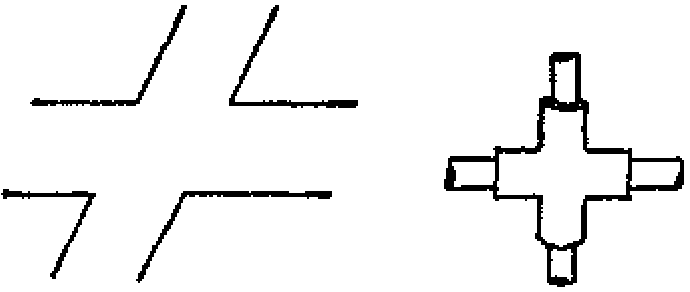
\includegraphics[width=5.5cm]{../pic/czjh1-ch2-01.png}
        \caption{}\label{fig:czjh1-2-1}
    \end{minipage}
    \qquad
    \begin{minipage}[b]{7cm}
        \centering
        \begin{tikzpicture}
	\tkzDefPoints{0/0/C, 4/0/B, 0/2/A, 4/2/D}
	\tkzInterLL(A,B)(C,D)   \tkzGetPoint{O}

	\tkzDrawSegments(A,B  C,D)

	\tkzMarkAngle[size=0.4](B,O,D)  \tkzLabelAngle[pos=0.7](B,O,D){$1$}
	\tkzMarkAngle[size=0.5](D,O,A)  \tkzLabelAngle[pos=0.8](D,O,A){$2$}
	\tkzMarkAngle[size=0.4](A,O,C)  \tkzLabelAngle[pos=0.7](A,O,C){$3$}
	\tkzMarkAngle[size=0.5](C,O,B)  \tkzLabelAngle[pos=0.8](C,O,B){$4$}

	\tkzLabelPoints[below](A, B, C, D, O)
\end{tikzpicture}


        \caption{}\label{fig:czjh1-2-2}
    \end{minipage}
\end{figure}


如图 \ref{fig:czjh1-2-2},直线 $AB$、$CD$ 相交于点 $O$,点 $O$ 把直线 $AB$、$CD$ 分成四条射线,
构成以点 $O$ 为顶点的四个角:$\angle 1$、$\angle 2$、$\angle 3$、 $\angle 4$。
其中 $\angle 1$ 的两边 $OB$、$OD$ 分别是 $\angle 3$ 的两边 $OA$、$OC$ 的反向延长线。
一个角的两边分别是另一个角的两边的反向延长线,这两个角叫做\zhongdian{对顶角}。
例如,$\angle 1$ 和 $\angle 3$ 是对顶角; 同样,$\angle 2$ 和 $\angle 4$ 也是对顶角。

对顶角有什么关系呢? 我们来看 $\angle 1$ 和 $\angle 3$。

因为 $AOB$ 是直线, 所以 $\angle 1$ 和 $\angle 2$ 是邻补角。

同理 $\angle 3$ 和 $\angle 2$ 也是邻补角。

根据同角的补角相等,所以 $\angle 1 = \angle 3$。

由此,我们得到对顶角的性质:

\begin{xingzhi}
    对顶角相等。
\end{xingzhi}

根据对顶角相等这个性质,已知 $\angle 2$ 和 $\angle 4$ 是对顶角(图 \ref{fig:czjh1-2-2}),
我们就可以得到 $\angle 2 = \angle 4$。可以写成:

$\because$ \quad $\angle 2$ 和 $\angle 4$ 是对顶角(已知),

$\therefore$ \quad $\angle 2 = \angle 4$(对顶角相等)。


\begin{lianxi}

口答下列各题:

\xiaoti{}%
\begin{xiaoxiaotis}%
    \xxt[\xxtsep]{图甲中点 $A$、$O$、$B$ 在一条直线上, 点 $C$、$O$、$D$ 不在一条直线上,$\angle 1$ 和 $\angle 2$ 是不是对顶角?为什么?}

    \xxt{图乙中点 $O$、$P$ 是不同的两点, $\angle 3$ 和 $\angle 4$ 是不是对顶角?为什么?}

    \xxt{怎么样的两个角才是对顶角?}

\end{xiaoxiaotis}


\begin{figure}[htbp]
    \centering
    \begin{minipage}[b]{7cm}
        \centering
        \begin{tikzpicture}
	\tkzDefPoints{0/0/A, 4/0/B, 0/1/C, 3/-1/D, 2/0/O}
	\tkzDrawSegments(A,B  C,O  O,D)

	\tkzMarkAngle[size=0.5](C,O,A)  \tkzLabelAngle[pos=0.8](C,O,A){$1$}
	\tkzMarkAngle[size=0.5](D,O,B)  \tkzLabelAngle[pos=0.8](D,O,B){$2$}

	\tkzLabelPoints[below](A, B, D)
	\tkzLabelPoints[left](C)
	\tkzLabelPoints[above](O)
\end{tikzpicture}


        \caption*{甲}
    \end{minipage}
    \qquad
    \begin{minipage}[b]{7cm}
        \centering
        \begin{tikzpicture}
	\tkzDefPoints{0/0/A, 4/0/B, 0/1/C, 4/-1/D, 1.5/0/O, 2.5/0/P}
	\tkzDrawSegments(A,B  C,O  P,D)

	\tkzMarkAngle[size=0.5](C,O,A)  \tkzLabelAngle[pos=0.8](C,O,A){$1$}
	\tkzMarkAngle[size=0.5](D,P,B)  \tkzLabelAngle[pos=0.8](D,P,B){$2$}

	\tkzLabelPoints[below](A, B, D, O)
	\tkzLabelPoints[left](C)
	\tkzLabelPoints[above](P)
\end{tikzpicture}


        \caption*{乙}
    \end{minipage}
    \caption*{(第 1 题)}
\end{figure}



\xiaoti{如图, $AB$、$CD$、$EF$ 是经过点 $O$ 的三条直线,说出 $\angle AOC$、$\angle FOB$ 的对顶角。}


\begin{figure}[htbp]
    \centering
    \begin{minipage}[b]{7cm}
        \centering
        \begin{tikzpicture}
	\tkzDefPoints{0/0/O, -2/0/A, 2/0/B, -1.5/1.5/C, 1.5/-1.5/D, -1.5/-1.5/F, 1.5/1.5/E}
	\tkzDrawSegments(A,B  C,D  E,F)

	\tkzLabelPoints[below](A, B, D, F, O)
	\tkzLabelPoints[left](C)
	\tkzLabelPoints[right](E)
\end{tikzpicture}


        \caption*{(第 2 题)}
    \end{minipage}
    \qquad
    \begin{minipage}[b]{7cm}
        \centering
        \begin{tikzpicture}
	\tkzDefPoints{0/0/A, 5/0/B, 0.4/2/C, 5/2/D, 0.5/-1/E, 4/3/F}
	\tkzInterLL(A,B)(E,F)   \tkzGetPoint{H}
	\tkzInterLL(C,D)(E,F)   \tkzGetPoint{G}

	\tkzDrawSegments(A,B  C,D  E,F)

	\tkzMarkAngle[size=0.4](D,G,F)  \tkzLabelAngle[pos=0.6](D,G,F){$1$}
	\tkzMarkAngle[size=0.3](F,G,C)  \tkzLabelAngle[pos=0.5](F,G,C){$2$}
	\tkzMarkAngle[size=0.4](C,G,E)  \tkzLabelAngle[pos=0.6](C,G,E){$3$}
	\tkzMarkAngle[size=0.3](E,G,D)  \tkzLabelAngle[pos=0.5](E,G,D){$4$}

	\tkzMarkAngle[size=0.4](B,H,F)  \tkzLabelAngle[pos=0.6](B,H,F){$5$}
	\tkzMarkAngle[size=0.3](F,H,A)  \tkzLabelAngle[pos=0.5](F,H,A){$6$}
	\tkzMarkAngle[size=0.4](A,H,E)  \tkzLabelAngle[pos=0.6](A,H,E){$7$}
	\tkzMarkAngle[size=0.3](E,H,B)  \tkzLabelAngle[pos=0.5](E,H,B){$8$}

	\tkzLabelSegment[pos=1.0, right](E,F){$l_1$}
	\tkzLabelSegment[pos=1.0, below](C,D){$l_2$}
	\tkzLabelSegment[pos=1.0, below](A,B){$l_3$}
\end{tikzpicture}


        \caption*{(第 3 题)}
    \end{minipage}
\end{figure}


\xiaoti{如图,直线 $l_1$ 截直线 $l_2$ 和 $l_3$,构成八个角。已知 $\angle 1 = \angle 5 = 60^\circ$。}
\begin{xiaoxiaotis}

    \begin{tblr}[]{columns={colsep=0pt}}
        \xxt{$\angle 3$ 等于多少度?为什么?} &  \xxt{$\angle 3$ 和 $\angle 5$ 等不等?} \\
        \xxt{$\angle 7$ 等于多少度?为什么?} &  \xxt{$\angle 3$ 和 $\angle 7$ 等不等?} \\
        \SetCell[c=2]{} \xxt{$\angle 2$ 和 $\angle 4$ 各等于多少度?为什么? $\angle 6$ 和 $\angle 8$ 呢?}
    \end{tblr}

\end{xiaoxiaotis}

\end{lianxi}

